\documentclass[a4paper]{article}

\usepackage{times}
\usepackage{tikz}
\usepackage[margin=0cm]{geometry}
\usepackage{graphicx}
\usepackage{anyfontsize}
\usepackage{fancyhdr}
\usepackage{indentfirst}
\usepackage{amsmath}
\usepackage[spanish]{babel}
\usepackage[utf8]{inputenc}

\author{}
\date{}
\title{}

\begin{document}
\thispagestyle{empty}

\begin{tikzpicture}[remember picture, overlay]
    \pgftransformshift{\pgfpoint{0cm}{0cm}}
    \draw [line width=2pt](1cm,-1cm) -- (1cm,-27.7cm) -- (14cm, -27.7cm) -- (14cm, -1cm) -- (1cm, -1cm);
    \draw[line width=2pt] (15cm, -27.7cm) -- (19cm,-27.7cm) -- (19cm, -1cm) -- (15cm, -1cm) --  (15cm, -27.7cm);
    \node [line width=2pt] at (17cm, -3.5cm) {
\includegraphics[width=3cm]{/home/marcosgatica/Imágenes/utn.png}};
		\node [line width=2pt] at (7.5cm, -7.5cm) {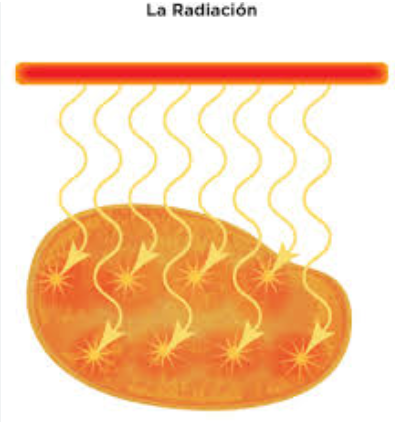
\includegraphics[width=6cm]{./imagenCaratula.png}};
    \node at (17cm, -7cm) {\scalebox{5}{\textbf{U}}};
    \node at (17cm, -9cm) {\scalebox{5}{\textbf{T}}};
    \node at (17cm, -11cm) {\scalebox{5}{\textbf{N}}};
    \node at (17cm, -14cm) {\scalebox{5}{\textbf{F}}};
    \node at (17cm, -16cm) {\scalebox{5}{\textbf{R}}};
    \node at (17cm, -18cm) {\scalebox{5}{\textbf{C}}};
    \node at (7.5cm, -12cm) {\scalebox{2.5}{\textbf{RADIACIÓN TÉRMICA}}};

    \node at (7.5cm, -24cm) {\begin{minipage}[c]{12cm}
        \raggedright
        \vspace{1.5cm}
        \fontsize{14}{14}\selectfont \textbf{Autor:} Marcos Raúl Gatica. \\
        \fontsize{14}{14}\selectfont \textbf{Curso:} 2R1. \\
        \fontsize{14}{14}\selectfont \textbf{Asignatura:} Física Electrónica. \\
        \fontsize{14}{14}\selectfont \textbf{Institución:} Universidad Tecnológica Nacional - Facultad Regional de Córdoba. \\

    \end{minipage}};

\end{tikzpicture}

\renewcommand{\normalsize}{\fontsize{12}{18}\selectfont}
\newgeometry{margin=1cm}
\fancyhf{}
\renewcommand{\headrulewidth}{0pt}
\renewcommand{\footrulewidth}{0pt}
\fancyfoot[R]{\textit{Gatica M. - Leg. 402006 - 2R1 pág. \thepage}}
\setlength{\footskip}{0pt}

\newpage
\newpage

\thispagestyle{empty}
\setcounter{page}{0}
\tableofcontents

\newpage
\thispagestyle{fancy}


\twocolumn
\flushbottom
\section{INTRODUCCIÓN}
    \subsection{La radiación térmica}
        \indent Se entiende como la radiación térmica al modo de transmitir calor de un sistema (la superficie de un cuerpo) al entorno. No requiere un medio para transmitirse, aunque es más eficaz la transmisión en el vacío. \\
        \indent Una superficie calentada a un temperatura finita interactua con el medio a menor temperatura y comienza la transmisión de calor, esto último es conocido como la radiación que emite un objeto más caliente que su entorno hasta alcanzar el equilibrio térmico. \\
        \indent La radiación que emite un sólido más caliente que su entorno se conoce como emisividad (\textbf{E}), proviene de la energía interna y la velocidad a la que la energía es emitida por la materia por su unidad de área (\textit{$\frac {W} {m^2}$}). \\

    \subsection{Radiación y las longitudes de onda}
        \indent La radiación térmica que emite un cuerpo caliente representa varias longitudes de onda. Gráficamente se puede ver que cada curva representa la variación de emisión monocromática con la long. de onda $\lambda$ \\

        \begin{tikzpicture}[remember picture, overlay]
        \node at (2.75cm, -2cm) {
            \begin{minipage}[c]{3cm}
                \includegraphics[width = 5.5cm]{./radiaciónTermVSLambda.png}
            \end{minipage}};
        \end{tikzpicture}
    \vspace{4.8cm}
    \subsection{Experimento y objetivos}
        El objetivo de este desarrollo de laboratorio es determinar la radiación térmica que emanan los siguientes materiales:
        \begin{itemize}
            \setlength{\itemsep}{0pt}
            \item Plomo 
            \item Aluminio anodizado
            \item Bronce
            \item Cobre 
            \item Chapa negra
        \end{itemize}
\end{document}


